\documentclass[11pt,a4paper]{article}

% ------------------------------------------------------------------
% Packages
% ------------------------------------------------------------------
\usepackage[T1]{fontenc}
\usepackage[utf8]{inputenc}
\usepackage{lmodern}
\usepackage[a4paper,margin=2.2cm]{geometry}
\usepackage{amsmath,amssymb}
\usepackage{xcolor}
\usepackage{tikz}
\usetikzlibrary{arrows.meta,positioning,decorations.pathreplacing,calc}
\usepackage{pgfgantt}
\usepackage{booktabs,tabularx,array,multirow}
\usepackage{enumitem}
\usepackage{algorithm}
\usepackage[noend]{algpseudocode}
\usepackage{caption}
\usepackage{float}
\usepackage[hidelinks]{hyperref}

\setlist{itemsep=2pt,topsep=3pt}
\captionsetup{font=small,labelfont=bf}
\renewcommand{\arraystretch}{1.15}

% ------------------------------------------------------------------
% Team data -- fill in once, used everywhere in the document
% ------------------------------------------------------------------
\newcommand{\PA}{Jakub Wilczyński}   % project coordinator
\newcommand{\PB}{Nylan Santos}
\newcommand{\PC}{Antoni Piałucha}
\newcommand{\PD}{Maksymilian Tulewicz}
\newcommand{\IA}{275459}
\newcommand{\IB}{300482}
\newcommand{\IC}{275411}
\newcommand{\ID}{275421}
\newcommand{\Instructor}{Gurjinder Singh}

% ------------------------------------------------------------------
% Notation
% ------------------------------------------------------------------
\newcommand{\ev}[1]{\mathsf{#1}}            % event names
\newcommand{\md}[1]{\textsc{#1}}            % robot modes
\newcommand{\EF}{\mathrm{EF}}
\newcommand{\Econ}{E_{\mathrm{con}}}
\newcommand{\Eobs}{E_{\mathrm{obs}}}
\newcommand{\Euc}{E_{\mathrm{uc}}}
\newcommand{\occ}{\mathrm{occ}}
\newcommand{\pos}{\mathrm{pos}}
\newcommand{\nxt}{\mathrm{next}}
\newcommand{\rest}{\mathrm{rest}}
\newcommand{\Bf}{\mathcal{B}}
\newcommand{\nil}{\bot}

% ------------------------------------------------------------------
% Layout drawing helpers (1 unit = 1 grid cell)
% ------------------------------------------------------------------
\definecolor{laneC}{gray}{0.93}
\definecolor{rackC}{RGB}{110,110,118}
\definecolor{pickC}{RGB}{120,190,120}
\definecolor{dropC}{RGB}{240,160,80}
\definecolor{chgC}{RGB}{110,160,230}
\definecolor{parkC}{RGB}{200,220,245}
\definecolor{xingC}{RGB}{250,225,120}
\definecolor{robotC}{RGB}{200,40,40}

\newcommand{\cell}[3]{\fill[#3] (#1,#2) rectangle ++(1,1);}
\newcommand{\aR}[2]{\draw[-{Stealth[length=1.3mm]},black!45] (#1+0.22,#2+0.5)--(#1+0.78,#2+0.5);}
\newcommand{\aL}[2]{\draw[-{Stealth[length=1.3mm]},black!45] (#1+0.78,#2+0.5)--(#1+0.22,#2+0.5);}
\newcommand{\aU}[2]{\draw[-{Stealth[length=1.3mm]},black!45] (#1+0.5,#2+0.22)--(#1+0.5,#2+0.78);}
\newcommand{\aD}[2]{\draw[-{Stealth[length=1.3mm]},black!45] (#1+0.5,#2+0.78)--(#1+0.5,#2+0.22);}
\newcommand{\robot}[3]{\node[circle,fill=robotC,text=white,inner sep=0pt,minimum size=4.6mm,font=\tiny\bfseries] at (#1+0.5,#2+0.5) {#3};}
\newcommand{\lbl}[3]{\node[font=\scriptsize\bfseries] at (#1+0.5,#2+0.5) {#3};}

% ------------------------------------------------------------------
\begin{document}

% ---------------------------- Title block -------------------------
\begin{center}
  {\small Wrocław University of Science and Technology \quad$\cdot$\quad Event-Based Control \quad$\cdot$\quad Project Proposal}\\[10pt]
  {\LARGE\bfseries Deadlock-Free Event-Based Coordination\\[3pt] of a Mobile Robot Fleet in a Grid Warehouse}\\[10pt]
  {\normalsize \PA{}, \PB{}, \PC{}, \PD{}}\\[3pt]
  {\small Instructor: \Instructor \qquad October 2026}
\end{center}
\vspace{4pt}
\hrule
\vspace{6pt}

% ==================================================================
\section{The Problem of the Project}
% ==================================================================

\paragraph{Subject.}
The project concerns the supervisory, event-based control of a fleet of
$10$ autonomous mobile robots (AGVs) operating in a small automated
warehouse. The warehouse floor is modelled as a grid of cells. Robots
travel along one-way aisles between \textbf{5 pick-up stations} located
at the storage racks, \textbf{3 delivery (outbound) stations},
\textbf{4 charging ports} and a \textbf{parking area}. Customer orders
arrive over time; each order requires a robot to collect a load at a
given pick-up station and bring it to a given delivery station
(Fig.~\ref{fig:layout}). Every grid cell is treated as a shared
resource with unit capacity: a robot must acquire the next cell before it
may enter it and releases the previous cell after leaving it.

\paragraph{Why it is important.}
Fleets of mobile robots are the backbone of modern intralogistics
(e.g.\ goods-to-person systems in e-commerce warehouses). When many robots
share narrow aisles and intersections, purely local obstacle avoidance is
not sufficient: robots can end up in a \emph{circular wait}, in which each
robot waits for a cell held by the next one, and the whole system stops
(\emph{deadlock}). Such situations are difficult to recover from
automatically and directly reduce throughput. Moreover, robots have
limited battery capacity, so transport tasks compete with charging for
robot time and for a small number of charging ports. These are typical
discrete-event phenomena: the relevant dynamics is the order of events
(a robot enters a cell, a load is picked, an order arrives, a battery is
charged), not the continuous motion itself. The problem is therefore a
natural application of the methods of event-based control:
finite-state / resource-allocation models, deadlock avoidance and
event prioritisation.

\paragraph{Expected result.}
\begin{enumerate}[leftmargin=*]
  \item A formal discrete-event model of the warehouse (state space,
        events, enabling function $\EF(s)$ and transition function
        $\mathit{next\_state}(s,e)$).
  \item A supervisor that admits only safe events: collision freedom,
        deadlock freedom (algorithm $\mathit{safe}(s,e)$ with a correctness
        argument) and no robot running out of energy away from a charger.
  \item A set of prioritisation rules (order assignment, conflicts at cells
        and intersections, charging policy) evaluated with respect to
        throughput and order lead time.
  \item A Python discrete-event simulator used for fast experiments and for
        an exhaustive reachability check on a reduced instance.
  \item A ROS~2 / Gazebo demonstration with 10 robots in the warehouse
        world, controlled by the same supervisor, plus a final report and
        a recorded demo.
\end{enumerate}

% ==================================================================
\section{Model and Control Concept}
% ==================================================================

\subsection{Warehouse layout and assumptions}

\begin{figure}[H]
\centering
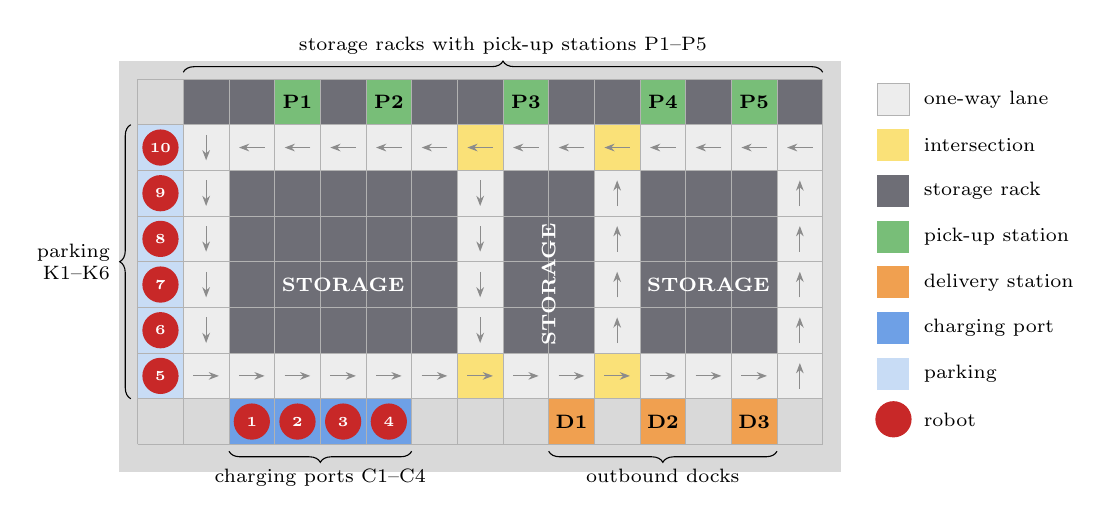
\begin{tikzpicture}[scale=0.58]
  % --- background / walls
  \fill[black!15] (0.6,0.4) rectangle (16.4,9.4);
  % --- lanes
  \foreach \x in {2,...,15} { \cell{\x}{7}{laneC} \cell{\x}{2}{laneC} }
  \foreach \y in {3,...,6} { \cell{2}{\y}{laneC} \cell{15}{\y}{laneC} \cell{8}{\y}{laneC} \cell{11}{\y}{laneC} }
  % --- intersections
  \foreach \p in {(8,7),(11,7),(8,2),(11,2)} { \fill[xingC] \p rectangle ++(1,1); }
  % --- interior storage racks
  \foreach \x in {3,...,7,9,10,12,13,14} { \foreach \y in {3,...,6} { \cell{\x}{\y}{rackC} } }
  % --- top storage racks with pick-up bays
  \foreach \x in {2,...,15} { \cell{\x}{8}{rackC} }
  \cell{4}{8}{pickC} \cell{6}{8}{pickC} \cell{9}{8}{pickC} \cell{12}{8}{pickC} \cell{14}{8}{pickC}
  % --- bottom row: chargers and delivery stations
  \foreach \x in {3,...,6} { \cell{\x}{1}{chgC} }
  \cell{10}{1}{dropC} \cell{12}{1}{dropC} \cell{14}{1}{dropC}
  % --- parking
  \foreach \y in {2,...,7} { \cell{1}{\y}{parkC} }
  % --- grid lines
  \draw[black!30,line width=0.25pt] (1,1) grid (16,9);
  % --- lane directions
  \foreach \x in {3,...,15} { \aL{\x}{7} }
  \aD{2}{7}
  \foreach \x in {2,...,14} { \aR{\x}{2} }
  \aU{15}{2}
  \foreach \y in {3,...,6} { \aD{2}{\y} \aU{15}{\y} \aD{8}{\y} \aU{11}{\y} }
  % --- labels
  \lbl{4}{8}{P1} \lbl{6}{8}{P2} \lbl{9}{8}{P3} \lbl{12}{8}{P4} \lbl{14}{8}{P5}
  \lbl{10}{1}{D1} \lbl{12}{1}{D2} \lbl{14}{1}{D3}
  \node[white,font=\scriptsize\bfseries] at (5.5,4.5) {STORAGE};
  \node[white,font=\scriptsize\bfseries,rotate=90] at (10,4.5) {STORAGE};
  \node[white,font=\scriptsize\bfseries] at (13.5,4.5) {STORAGE};
  % --- robots in the initial state s0
  \robot{3}{1}{1} \robot{4}{1}{2} \robot{5}{1}{3} \robot{6}{1}{4}
  \robot{1}{2}{5} \robot{1}{3}{6} \robot{1}{4}{7} \robot{1}{5}{8} \robot{1}{6}{9} \robot{1}{7}{10}
  % --- braces / annotations
  \draw[decorate,decoration={brace,amplitude=4pt,mirror}] (3,0.85)--(7,0.85) node[midway,below=3pt,font=\scriptsize]{charging ports C1--C4};
  \draw[decorate,decoration={brace,amplitude=4pt,mirror}] (10,0.85)--(15,0.85) node[midway,below=3pt,font=\scriptsize]{outbound docks};
  \draw[decorate,decoration={brace,amplitude=4pt}] (0.85,2)--(0.85,8) node[midway,left=4pt,font=\scriptsize,align=right]{parking\\K1--K6};
  \draw[decorate,decoration={brace,amplitude=4pt}] (2,9.15)--(16,9.15) node[midway,above=3pt,font=\scriptsize]{storage racks with pick-up stations P1--P5};
  % --- legend
  \begin{scope}[shift={(17.2,2.2)},font=\scriptsize]
    \fill[laneC] (0,6) rectangle ++(0.7,0.7); \draw[black!30] (0,6) rectangle ++(0.7,0.7); \node[right] at (0.8,6.35) {one-way lane};
    \fill[xingC] (0,5) rectangle ++(0.7,0.7); \node[right] at (0.8,5.35) {intersection};
    \fill[rackC] (0,4) rectangle ++(0.7,0.7); \node[right] at (0.8,4.35) {storage rack};
    \fill[pickC] (0,3) rectangle ++(0.7,0.7); \node[right] at (0.8,3.35) {pick-up station};
    \fill[dropC] (0,2) rectangle ++(0.7,0.7); \node[right] at (0.8,2.35) {delivery station};
    \fill[chgC]  (0,1) rectangle ++(0.7,0.7); \node[right] at (0.8,1.35) {charging port};
    \fill[parkC] (0,0) rectangle ++(0.7,0.7); \node[right] at (0.8,0.35) {parking};
    \node[circle,fill=robotC,inner sep=0pt,minimum size=4.6mm] at (0.35,-0.65) {}; \node[right] at (0.8,-0.65) {robot};
  \end{scope}
\end{tikzpicture}
\caption{Proposed warehouse layout ($15\times 8$ cells). Lanes form a
one-way loop with two cross connectors, creating four intersections.
Stations, charging ports and parking places are dead-end \emph{buffer
cells}. The robots are shown in the initial state $s_0$.}
\label{fig:layout}
\end{figure}

\noindent Modelling assumptions:
\begin{itemize}[leftmargin=*]
  \item The floor is a set of cells $V$; a cell is $1\times1$\,m and can
        hold at most one robot. $V = L \cup \Bf$, where $L$ are lane cells
        ($|L|=44$) and $\Bf = P\cup D\cup C\cup K$ are buffer cells:
        pick-up stations $P=\{p_1,\dots,p_5\}$, delivery stations
        $D=\{d_1,d_2,d_3\}$, charging ports $C=\{c_1,\dots,c_4\}$ and parking
        places $K=\{k_1,\dots,k_6\}$. The number of home cells
        $|C\cup K| = 10$ equals the fleet size, so every robot always has a
        place to go when it is idle.
  \item Admissible moves are given by a directed graph $G=(V,A)$ that encodes
        the lane directions of Fig.~\ref{fig:layout}. Every buffer cell is a
        dead end connected to exactly one lane cell (in and out). For
        every pair of cells, $\mathit{route}(u,g)$ is a fixed shortest path
        in $G$ and $\delta(u,g)$ is its length (number of moves).
  \item Robots $R=\{1,\dots,10\}$ carry at most one load. Loading, unloading
        and charging take a finite, not exactly known time.
  \item An order $o=(p_o,d_o)$, $p_o\in P$, $d_o\in D$, is generated by the
        warehouse management system at unknown times. The battery level is
        measured in moves: one move costs one unit, full capacity is $B$
        (e.g.\ $B=400$), and $b_{\mathrm{res}}$ is a safety reserve.
\end{itemize}

% ------------------------------------------------------------------
\subsection{System state}

The state of robot $i\in R$ is the tuple
\[
  s_i = (H_i,\; m_i,\; b_i,\; o_i,\; g_i),
\]
where
\begin{itemize}[leftmargin=*]
  \item $H_i$ -- the sequence of cells held by the robot: $H_i=(u)$ when the
        robot stands in cell $u$, $H_i=(u,v)$ while it moves from $u$ to $v$
        (it holds both cells). We write $\pos_i=u$ for the first element;
  \item $m_i \in M$ -- the operating mode (Fig.~\ref{fig:modes}), where
        $M = \{\md{Idle}, \md{ToPick}, \md{Loading}, \md{Loaded}, \md{ToDrop},$
        $\md{Unloading}, \md{ToCharge}, \md{Charging}, \md{ToPark}\}$;
  \item $b_i\in\{0,\dots,B\}$ -- battery level;
  \item $o_i \in \mathcal{O}\cup\{\nil\}$ -- the order assigned to the robot;
  \item $g_i \in \Bf\cup\{\nil\}$ -- the goal buffer cell, reserved for robot $i$
        until it arrives there.
\end{itemize}
The symbol $\nil$ means ``none'': $o_i=\nil$ -- the robot has no order,
$g_i=\nil$ -- the robot has no reserved goal (it is not driving anywhere).
The system state is $s = (s_1,\dots,s_{10},\,Q,\,n)$, where $Q$ is the FIFO
queue of unassigned orders ($|Q|\le Q_{\max}$) and $n$ is the number of
delivered orders. The state space $S$ is the set of all such tuples that
satisfy the structural constraints (at most one robot per cell, at most one
reservation per buffer cell). Derived quantities used below:
$\occ(v)=i$ if $v\in H_i$ and $\nil$ otherwise; $\mathit{free}(g)\iff
\occ(g)=\nil \wedge \neg\exists j\colon g_j=g$; $\nxt_i$ is the second cell of
$\mathit{route}(\pos_i,g_i)$ and $\rest_i$ is the set of cells of this route
not yet held by robot $i$.

Even with the routes fixed, $|S|$ grows roughly as $|V|^{10}$
($|V|=62$), i.e.\ well above $10^{17}$, so the full model is not analysed by
enumeration. Correctness is enforced on-line by the supervisor
(Sec.~\ref{sec:safety}) and checked exhaustively only on a reduced instance.

\paragraph{Initial state $s_0$.} Robots 1--4 stand on charging ports
$c_1,\dots,c_4$ and robots 5--10 on parking places $k_1,\dots,k_6$; for all
$i$: $m_i=\md{Idle}$, $b_i=B$, $o_i=\nil$, $g_i=\nil$; $Q=\emptyset$
(continuous operation) or $Q=Q_0$, a given batch of $N$ orders (batch
scenario); $n=0$.

\paragraph{Final state $s_{\mathrm{fin}}$} (batch scenario only).
$Q=\emptyset$, $n=N$, and every robot is \md{Idle} on a charging port or a
parking place. In continuous operation no final state is defined; liveness is
used instead (Sec.~\ref{sec:safety}).

% ------------------------------------------------------------------
\subsection{Events}

All events are parameterised by robot, order or cell. Controllable events are
commands issued by the supervisor; uncontrollable events are reported by the
robots or by the warehouse management system.

\begin{table}[H]
\centering\small
\begin{tabularx}{\textwidth}{@{}l c X@{}}
\toprule
Event & Type & Meaning \\
\midrule
$\ev{order}(o)$         & uc & a new order $o=(p_o,d_o)$ arrives from the WMS \\
$\ev{assign}(i,o)$      & c  & order $o$ is assigned to robot $i$ \\
$\ev{dispatch}(i,g)$    & c  & robot $i$ is given goal buffer cell $g$, which is reserved for it \\
$\ev{enter}(i,v)$       & c  & robot $i$ is allowed to start moving into the neighbouring cell $v$ \\
$\ev{arrive}(i)$        & uc & robot $i$ has completed the move and released the previous cell \\
$\ev{load}(i)$, $\ev{unload}(i)$ & c & start of loading at $p_{o_i}$ / unloading at $d_{o_i}$ \\
$\ev{loaded}(i)$, $\ev{unloaded}(i)$ & uc & end of loading / unloading \\
$\ev{charge}(i)$        & c  & start of charging \\
$\ev{charged}(i)$       & uc & battery full, charging finished \\
\bottomrule
\end{tabularx}
\caption{Events (c -- controllable, uc -- uncontrollable).}
\label{tab:events}
\end{table}

Hence (with all parameter values)
\begin{align*}
  \Econ &= \{\ev{assign},\ev{dispatch},\ev{enter},\ev{load},\ev{unload},\ev{charge}\},\\
  \Euc  &= \{\ev{order},\ev{arrive},\ev{loaded},\ev{unloaded},\ev{charged}\}.
\end{align*} In the basic model all events are observable,
$\Eobs = E = \Econ\cup\Euc$: robots report the completion of each move and
each operation, and the WMS reports new orders. The continuous pose of a
robot between two cells is not observed by the supervisor; it is abstracted
away by the pair $\ev{enter}$/$\ev{arrive}$. As an optional extension we may
add the observable but uncontrollable event $\ev{fault}(i)$ (robot stopped by
an obstacle or failure), which turns the cells held by robot $i$ into
temporarily blocked resources.

\begin{figure}[H]
\centering
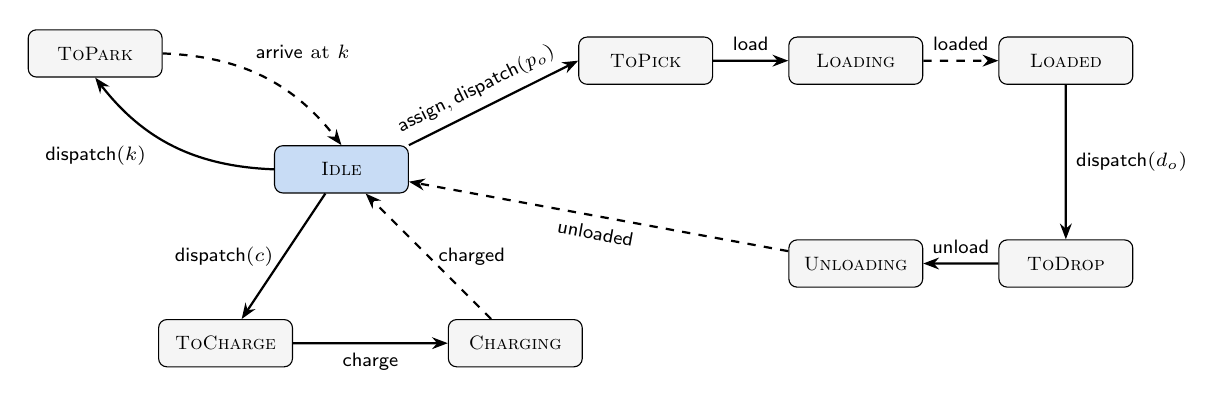
\begin{tikzpicture}[scale=0.92,>={Stealth[length=2mm]},font=\scriptsize,
  st/.style={draw,rounded corners=3pt,minimum width=17mm,minimum height=6mm,fill=black!4},
  c/.style={->,thick},u/.style={->,thick,dashed}]
  \node[st,fill=parkC] (idle) at (0,0) {\md{Idle}};
  \node[st] (tp)  at (4.2,1.5)  {\md{ToPick}};
  \node[st] (ld)  at (7.1,1.5)  {\md{Loading}};
  \node[st] (lo)  at (10.0,1.5)  {\md{Loaded}};
  \node[st] (td)  at (10.0,-1.3) {\md{ToDrop}};
  \node[st] (ul)  at (7.1,-1.3) {\md{Unloading}};
  \node[st] (tc)  at (-1.6,-2.4) {\md{ToCharge}};
  \node[st] (ch)  at (2.4,-2.4)  {\md{Charging}};
  \node[st] (tk)  at (-3.4,1.6)  {\md{ToPark}};
  \draw[c] (idle.north east) -- node[above,sloped,pos=0.45]{$\ev{assign},\ev{dispatch}(p_o)$} (tp.west);
  \draw[c] (tp) -- node[above]{$\ev{load}$} (ld);
  \draw[u] (ld) -- node[above]{$\ev{loaded}$} (lo);
  \draw[c] (lo) -- node[right]{$\ev{dispatch}(d_o)$} (td);
  \draw[c] (td) -- node[above]{$\ev{unload}$} (ul);
  \draw[u] (ul) -- node[below,sloped]{$\ev{unloaded}$} (idle);
  \draw[c] (idle) -- node[left]{$\ev{dispatch}(c)$} (tc);
  \draw[c] (tc) -- node[below]{$\ev{charge}$} (ch);
  \draw[u] (ch) -- node[right]{$\ev{charged}$} (idle);
  \draw[c] (idle.west) to[bend left=25] node[below left,pos=0.6]{$\ev{dispatch}(k)$} (tk.south);
  \draw[u] (tk.east) to[bend left=25] node[above right,pos=0.4]{$\ev{arrive}$ at $k$} (idle.north);
\end{tikzpicture}
\caption{Mode automaton of a single robot (solid -- controllable, dashed --
uncontrollable). In the modes \md{ToPick}, \md{ToDrop}, \md{ToCharge},
\md{ToPark} the robot repeats $\ev{enter}$/$\ev{arrive}$ along its route; this
is where robots interact through the shared cells.}
\label{fig:modes}
\end{figure}

% ------------------------------------------------------------------
\subsection{Events possible in a state}

$\EF(s)$ is the set of events that can occur in state $s$. Each event has a
\emph{guard}, i.e.\ an enabling condition on the state; for example,
$\ev{enter}(i,v)$ requires that cell $v$ is free. An event $e$ belongs to
$\EF(s)$ if and only if its guard in Table~\ref{tab:transitions} (column
``Guard'') is true in $s$. The guards are
local and cheap to evaluate, so $\EF(s)$ is computed by a simple loop over
robots, orders and buffer cells. Let
$M_{\mathrm{mov}}=\{\md{ToPick},\md{ToDrop},\md{ToCharge},\md{ToPark}\}$ and
let the energy-feasibility test be
\[
  \mathit{feas}(i,o) \iff b_i \ge \delta(\pos_i,p_o)+\delta(p_o,d_o)
  +\max_{c\in C}\delta(d_o,c) + b_{\mathrm{res}} .
\]

Two observations: (i) the guard of $\ev{enter}(i,v)$ already excludes
collisions, since $v$ must be unoccupied, and buffer cells can be entered only
by the robot that reserved them; (ii) $\EF(s)$ only describes what is
\emph{physically and logically possible}. The supervisor further restricts
the controllable events with $\mathit{safe}(s,e)$ (Sec.~\ref{sec:safety}) and
chooses among the remaining ones with the priority rules
(Sec.~\ref{sec:priority}).

% ------------------------------------------------------------------
\subsection{State transition}

The transition function $s'=\mathit{next\_state}(s,e)$, defined for
$e\in\EF(s)$, is given in the column ``Effect'' of
Table~\ref{tab:transitions}. Variables not mentioned remain unchanged.

\begin{table}[H]
\centering\small
\begin{tabularx}{\textwidth}{@{}p{2.3cm} X X@{}}
\toprule
Event $e$ & Guard: $e\in\EF(s)$ iff & Effect: $s'=\mathit{next\_state}(s,e)$\\
\midrule
$\ev{order}(o)$ & $|Q|<Q_{\max}$ & $Q \leftarrow Q\cdot o$ (append) \\
$\ev{assign}(i,o)$ & $o\in Q$, $m_i=\md{Idle}$, $o_i=\nil$, $|H_i|=1$, $\pos_i\in C\cup K$, $\mathit{feas}(i,o)$ & $o_i\leftarrow o$, $Q\leftarrow Q\setminus\{o\}$ \\
$\ev{dispatch}(i,g)$ & $|H_i|=1$, $\pos_i\in\Bf$, $\mathit{free}(g)$ and one of:
  (a) $m_i=\md{Idle}$, $o_i\neq\nil$, $g=p_{o_i}$;
  (b) $m_i=\md{Loaded}$, $g=d_{o_i}$;
  (c) $m_i=\md{Idle}$, $o_i=\nil$, $g\in C$, $b_i\ge\delta(\pos_i,g)$;
  (d) $m_i=\md{Idle}$, $o_i=\nil$, $g\in K$, $b_i\ge\delta(\pos_i,g)+\delta(g,C)$
  & $g_i\leftarrow g$; $m_i\leftarrow$ (a) \md{ToPick}, (b) \md{ToDrop}, (c) \md{ToCharge}, (d) \md{ToPark} \\
$\ev{enter}(i,v)$ & $m_i\in M_{\mathrm{mov}}$, $g_i\neq\nil$, $|H_i|=1$, $v=\nxt_i$, $\occ(v)=\nil$, $b_i\ge 1$ & $H_i\leftarrow(\pos_i,v)$ \\
$\ev{arrive}(i)$ & $H_i=(u,v)$ & $H_i\leftarrow(v)$, $b_i\leftarrow b_i-1$; if $v=g_i$: $g_i\leftarrow\nil$ and, if $m_i=\md{ToPark}$, $m_i\leftarrow\md{Idle}$ \\
$\ev{load}(i)$ & $m_i=\md{ToPick}$, $H_i=(p_{o_i})$ & $m_i\leftarrow\md{Loading}$ \\
$\ev{loaded}(i)$ & $m_i=\md{Loading}$ & $m_i\leftarrow\md{Loaded}$ \\
$\ev{unload}(i)$ & $m_i=\md{ToDrop}$, $H_i=(d_{o_i})$ & $m_i\leftarrow\md{Unloading}$ \\
$\ev{unloaded}(i)$ & $m_i=\md{Unloading}$ & $m_i\leftarrow\md{Idle}$, $o_i\leftarrow\nil$, $n\leftarrow n+1$ \\
$\ev{charge}(i)$ & $m_i=\md{ToCharge}$, $H_i=(c)$, $c\in C$, $g_i=\nil$ & $m_i\leftarrow\md{Charging}$ \\
$\ev{charged}(i)$ & $m_i=\md{Charging}$ & $m_i\leftarrow\md{Idle}$, $b_i\leftarrow B$ \\
\bottomrule
\end{tabularx}
\caption{Enabling function $\EF(s)$ and transition function $\mathit{next\_state}(s,e)$.}
\label{tab:transitions}
\end{table}

The condition $g_i=\nil$ in the guard of $\ev{charge}(i)$ means that the robot
has reached its goal. Without it, a robot standing on one charger and heading
to another could start charging at once and keep its reservation of the other
charger.

% ------------------------------------------------------------------
\subsection{Correctness and safety}\label{sec:safety}

The behaviour of the system is considered correct if the following properties
hold in every state reachable under the supervisor.
\begin{enumerate}[label=\textbf{(S\arabic*)},leftmargin=*]
  \item \textbf{Collision freedom:} $H_i\cap H_j=\emptyset$ for all $i\neq j$.
  \item \textbf{Energy safety:} a robot never runs out of energy away from a
        charging port, i.e.\ $b_i\ge\delta(\pos_i,C)$ at all times.
  \item \textbf{Deadlock freedom:} there is no set of moving robots in which
        each robot waits for a cell held by another robot of the set
        (circular wait).
  \item[\textbf{(L)}] \textbf{Liveness / reachability:} every order in $Q$ is
        eventually delivered; in the batch scenario $s_{\mathrm{fin}}$ is
        reachable from every reachable state (the supervised system is
        non-blocking).
\end{enumerate}

(S1) and (S2) follow from the guards by induction over events: $s_0$
satisfies both, $\ev{enter}$ only acquires an unoccupied cell, buffer cells
are reserved exclusively, $\ev{arrive}$ only releases cells, and
$\mathit{feas}(i,o)$ guarantees enough energy to finish the order and reach
any charger. The energy conditions of $\ev{dispatch}$ (c) and (d) give the same
guarantee to a robot without an order: it can reach the chosen charger, or the
chosen parking place and then the nearest charger from there. (S3) does not follow from the guards: robots on the one-way loop
can fill a cycle of cells and block each other. It is enforced by a
\emph{deadlock-avoidance} test in the spirit of the Banker's algorithm for
resource allocation systems, applied to each controllable event before it is
issued.

\begin{algorithm}[H]
\caption{$\mathit{safe}(s,e)$ -- deadlock-avoidance test}\label{alg:safe}
\begin{algorithmic}[1]
\If{$e$ is not of the form $\ev{enter}(i,v)$} \Return \textbf{true}
  \Comment{other events do not acquire lane cells}
\EndIf
\State $s' \gets \mathit{next\_state}(s,e)$
\State $\mathcal{A} \gets \{\, j\in R : H_j \not\subseteq \Bf \,\}$
  \Comment{robots currently holding a lane cell}
\State $F \gets V \setminus \bigcup_{j\in\mathcal{A}} H_j$
  \Comment{cells not held by active robots}
\Repeat
  \State find $j\in\mathcal{A}$ such that $\rest_j \subseteq F$
     \Comment{$j$ can reach its reserved goal}
  \If{such $j$ exists}
     \State $\mathcal{A}\gets\mathcal{A}\setminus\{j\}$;\; $F\gets F\cup H_j$
       \Comment{$j$ parks in its buffer cell and frees its cells}
  \EndIf
\Until{no such $j$ exists}
\State \Return $(\mathcal{A}=\emptyset)$
\end{algorithmic}
\end{algorithm}

\paragraph{Proof idea.} Call a state \emph{safe} if Algorithm~\ref{alg:safe}
(the loop part) empties $\mathcal{A}$, i.e.\ there is an order in which all
active robots can drive to their reserved goal cells one after another.
(1) $s_0$ is safe, because all robots are in buffer cells.
(2) The supervisor issues a controllable event only if $\mathit{safe}(s,e)$
holds, so the next state is safe.
(3) Uncontrollable events cannot destroy safety: $\ev{arrive}$ only releases a
cell and shortens $\rest_i$, so the old completion order is still valid;
the other uncontrollable events do not change any $H_j$ or $\rest_j$.
Hence all reachable states are safe. In a safe state the first robot of the
completion order can always move, since its next cell is free, so a circular
wait cannot occur (S3). A robot that reaches its goal stands in a dead-end
buffer cell that lies on no other route, so it never blocks other robots.
Together with the station rule below, fairness (every started motion or
operation ends in finite time) and the aging rule of
Sec.~\ref{sec:priority}, which prevents starvation of robots waiting to leave
a buffer cell, this gives (L).
The test runs in $O(|R|^2\,\ell)$ time, where $\ell$ is the maximum route
length, which is negligible for 10 robots. The test is conservative
(sufficient but not necessary); a less restrictive variant that claims cells
only up to the next intersection will be compared experimentally.

\paragraph{Station rule.} Algorithm~\ref{alg:safe} checks only $\ev{enter}$
and only robots that hold a lane cell, so it cannot prevent blocking between
robots standing on stations. If a robot on a delivery station $d$ could accept
an order with pick-up $p$ while $p$ is held by a loaded robot whose order goes
to $d$, neither robot could ever be dispatched, because $\mathit{free}(p)$ and
$\mathit{free}(d)$ would both stay false. The condition $\pos_i\in C\cup K$ in
the guard of $\ev{assign}(i,o)$ excludes this situation: a robot that finishes
unloading has no order, so it can leave the station with $\ev{dispatch}$ (c)
or (d), and a robot that waits for a free pick-up station stands on a charger
or a parking place, where it does not block any station.

\paragraph{Demonstration of correctness.}
\begin{enumerate}[leftmargin=*]
  \item The invariant-based proof above, written in full in the report.
  \item \textbf{Exhaustive reachability analysis} on a reduced instance
        (e.g.\ 3--4 robots on a smaller version of the layout) with a BFS over
        the state graph generated by $\EF$ and $\mathit{next\_state}$.
        Without the supervisor, the analysis is expected to find reachable
        deadlock states (shown as counterexample traces). With
        $\mathit{safe}(s,e)$, no deadlock or collision state must be
        reachable, and $s_{\mathrm{fin}}$ must be reachable from every state.
  \item \textbf{Runtime monitors} in the 10-robot simulations that check
        (S1)--(S3) after every event and log every violation (target: zero
        violations over long randomised runs).
\end{enumerate}

% ------------------------------------------------------------------
\subsection{Event prioritisation and efficiency}\label{sec:priority}

\paragraph{Efficiency criterion.} The primary criterion is the
\textbf{throughput} $\Theta = n/T$ (orders delivered per hour of operation).
Secondary criteria are the mean and maximum \textbf{order lead time} (time
from $\ev{order}(o)$ to $\ev{unloaded}$ for $o$), the total time robots spend
blocked waiting for cells, and fleet utilisation.

\paragraph{Conflicts.} Typical conflicting events in one state are:
two robots requesting the same cell, i.e.\ $\ev{enter}(i,v)$ and $\ev{enter}(j,v)$,
one order that could be assigned to several robots, several robots competing
for one charging port, and several robots that want to leave buffer cells into
the same lane. In each state the supervisor first computes the candidate
set $\{e\in\Econ\cap\EF(s) : \mathit{safe}(s,e)\}$ and then applies
the rules below.
\begin{enumerate}[label=\textbf{R\arabic*.},leftmargin=*]
  \item \textbf{Cell conflicts.} Priority classes, from highest:
        (1) robot with critical battery ($b_i<b_{\mathrm{crit}}$) heading to a
        charger; (2) loaded robot (\md{ToDrop}); (3) robot already on the lane
        before a robot leaving a buffer cell (``main road first''); (4)
        \md{ToPick}; (5) \md{ToPark} and non-critical \md{ToCharge}.
        Within a class the robot with the longest waiting time wins
        (\emph{aging}, which prevents starvation); remaining ties are broken by
        robot index.
  \item \textbf{Intersections.} A robot may enter an intersection cell only if
        it can also take the cell behind the intersection (``do not block the
        box''). This is a cheap pre-filter for the $\mathit{safe}$ test.
  \item \textbf{Order assignment.} Orders are served in FIFO order, and
        overdue orders are moved forward. Each order is assigned to the idle
        robot on a charger or parking place with the smallest
        $\delta(\pos_i,p_o)$ that satisfies $\mathit{feas}(i,o)$. When several orders and robots are free at the
        same time, a minimum-cost assignment (Hungarian algorithm) can be
        used instead.
  \item \textbf{Charging policy.} If $b_i<b_{\mathrm{low}}$, charging takes
        priority over new orders for robot $i$. Idle robots with
        $b_i<b_{\mathrm{opp}}$ charge opportunistically when a port is free;
        otherwise idle robots go to parking.
  \item \textbf{Station clearing.} An idle robot standing in a pick-up or
        delivery station is dispatched away before robots in parking places
        are moved, so that stations are free for the next orders.
\end{enumerate}

\paragraph{Use for efficiency.} The rules reduce the time loaded robots spend
waiting and keep stations and intersections free, which shortens order lead
times. They also spread charging over idle periods, so fewer robots are
unavailable during peaks. The benefit will be quantified by comparing the
proposed policy with a baseline (first-come-first-served cell access, random
idle robot, charging only when the battery is low) at several order arrival
rates, using the same random order sequences for both policies.

% ------------------------------------------------------------------
\subsection{Proposed modelling approach}

The system is modelled as a \textbf{Resource Allocation System (RAS)}
expressed as a \textbf{finite-state automaton}: grid cells are reusable
resources of unit capacity, robots are processes that acquire and release
these resources in the sequence given by their routes, and the state
is the vector described above. This choice is appropriate because:
(i) deadlock in AGV systems is exactly a circular-wait problem of a RAS, so
established deadlock-avoidance theory (Banker-type safety tests) applies
directly; (ii) the model is finite, so $\EF$ and $\mathit{next\_state}$
can be executed directly as code, and the reduced instance can be checked by
enumeration; (iii) the same model can be translated into an equivalent Petri
net (cells as places with one token, robot moves as transitions), which we
will use for presentation and, if time permits, for structural analysis
(siphons) with an existing Petri-net tool.

% ------------------------------------------------------------------
\subsection{Planned implementation}

\begin{itemize}[leftmargin=*]
  \item \textbf{Model core} (Python 3): grid and route definitions, $\EF$,
        $\mathit{next\_state}$, $\mathit{safe}$ and the priority rules, as one
        library with unit tests (pytest).
  \item \textbf{Discrete-event simulator} (Python): random order streams and
        random operation times, KPI logging, the reachability analysis
        of the reduced instance, and policy comparison (plots with
        matplotlib).
  \item \textbf{ROS~2 (Humble/Jazzy) + Gazebo}: a warehouse world generated from
        the same grid description, 10 lightweight differential-drive
        robots, a robot-level node that executes cell-to-cell motion and
        publishes $\ev{arrive}$, $\ev{loaded}$, \dots{} events, and a
        \texttt{fleet\_supervisor} node that runs the model core and issues
        controllable events. Visualisation of states and reservations in RViz.
        Lightweight robot models keep the simulation real-time on standard
        laptops without a dedicated GPU.
  \item \textbf{Tools}: Git/GitHub, Overleaf (\LaTeX) for reports,
        recorded demo video.
\end{itemize}

% ==================================================================
\section{Work Plan and Timetable}
% ==================================================================

The project is planned for 10 weeks. Week 1 starts on 19 October 2026 and
the work is completed before the winter break. Exact milestone dates will be
aligned with the course schedule.

\begin{table}[H]
\centering\small
\begin{tabularx}{\textwidth}{@{}l X l l@{}}
\toprule
& Task & Responsible & Weeks \\
\midrule
T1 & Literature (RAS, AGV deadlock avoidance), requirements, layout & all (lead: A) & 1 \\
T2 & Formal model: state, events, $\EF$, $\mathit{next\_state}$ & A, B & 1--3 \\
T3 & Safety: $\mathit{safe}(s,e)$, invariant proof & B & 2--4 \\
T4 & Python model core, DES simulator, reachability analysis & B, C & 3--5 \\
T5 & Gazebo warehouse world and robot models & C & 2--5 \\
T6 & ROS~2 robot-level nodes (motion, event reporting, battery) & D & 3--6 \\
T7 & \texttt{fleet\_supervisor} node, integration of 10 robots & A, D & 6--8 \\
T8 & Priority policies, experiments, KPI evaluation & C, A & 7--9 \\
T9 & Reports, demo video, final presentation & all (lead: A) & 1, 5, 9--10 \\
\bottomrule
\end{tabularx}
\end{table}

\begin{figure}[H]
\centering
\begin{ganttchart}[
    hgrid, vgrid,
    x unit=0.95cm, y unit chart=0.46cm, y unit title=0.5cm,
    title label font=\scriptsize, bar label font=\scriptsize,
    milestone label font=\scriptsize\bfseries,
    bar/.append style={fill=chgC!80},
    milestone/.append style={fill=robotC},
    bar height=0.55, milestone height=0.6,
    inline=false
  ]{1}{10}
  \gantttitle{Oct}{2}\gantttitle{November}{4}\gantttitle{December}{4}\\
  \gantttitlelist{1,...,10}{1}\\
  \ganttbar{T1 Literature, requirements}{1}{1}\\
  \ganttbar{T2 Formal model}{1}{3}\\
  \ganttbar{T3 Safety, proof}{2}{4}\\
  \ganttbar{T4 Simulator, verification}{3}{5}\\
  \ganttbar{T5 Gazebo world}{2}{5}\\
  \ganttbar{T6 Robot-level nodes}{3}{6}\\
  \ganttbar{T7 Supervisor, integration}{6}{8}\\
  \ganttbar{T8 Policies, experiments}{7}{9}\\
  \ganttbar{T9 Reports}{1}{1}\ganttbar{}{5}{5}\ganttbar{}{9}{10}\\
  \ganttmilestone{M1 Proposal}{1}\\
  \ganttmilestone{M2 Model verified}{5}\\
  \ganttmilestone{M3 10-robot demo}{8}\\
  \ganttmilestone{M4 Final report}{10}
\end{ganttchart}
\caption{Gantt chart (weeks of the semester).}
\end{figure}

\noindent\textbf{Milestones:}
\textbf{M1} (week 1, 20 Oct 2026) -- proposal submitted;
\textbf{M2} (week 5, 20 Nov 2026) -- formal model, simulator and safety
verification on the reduced instance;
\textbf{M3} (week 8, 11 Dec 2026) -- 10-robot ROS~2/Gazebo demonstration;
\textbf{M4} (week 10, 22 Dec 2026) -- final report and presentation.

% ==================================================================
\section{Delivery}
% ==================================================================

\begin{itemize}[leftmargin=*]
  \item \textbf{M1 -- Proposal report} (this document): problem, model and
        control concept, plan. PDF and hard copy.
  \item \textbf{M2 -- Interim report}: complete formal model, $\mathit{safe}$
        algorithm with proof, reachability results (including the deadlock
        counterexample without the supervisor), first simulator KPIs.
        Attachment: archive (Git tag \texttt{m2}) with the model core,
        simulator and tests.
  \item \textbf{M3 -- Demonstration}: live or recorded demo of 10 robots in
        Gazebo with a short status note. Attachment: Git tag \texttt{m3}, ROS~2
        packages, launch files, demo video.
  \item \textbf{M4 -- Final report}: full description, policy comparison,
        conclusions, user guide. Attachments: final source archive (tag
        \texttt{v1.0}), simulation logs, plots and video. PDF.
\end{itemize}
\textbf{Disclosure:} reports are intended for the instructor and the team.
The source code is kept in a private repository during the semester and may
be published under the MIT licence after grading, with the consent of all
members.

% ==================================================================
\section{Project Management}
% ==================================================================

\begin{itemize}[leftmargin=*]
  \item \textbf{Structure and coordination.} The coordinator (\PA) assigns
        tasks, sets internal deadlines, merges changes into the main branch,
        and is the contact person for the instructor. Each task has one
        responsible member (Sec.~\ref{sec:team}).
  \item \textbf{Meetings and monitoring.} A weekly 30-minute online stand-up
        (Monday evening) reviews the status of each task on a GitHub Projects
        board (issues per task, \emph{To do / In progress / Review / Done}).
        Milestone readiness is reviewed one week before each milestone.
        Consultations with the instructor take place at milestones or on
        request.
  \item \textbf{Documents and communication.} Code on GitHub, reports in a
        shared Overleaf project, other files in a shared Google Drive folder.
        Day-to-day communication on a team Discord server; messages are
        answered within 24\,h on working days.
  \item \textbf{Software development rules.} Feature branches and pull
        requests; every pull request is reviewed by at least one other member
        and must pass automated tests (GitHub Actions, pytest, linter);
        PEP\,8 and ROS~2 package conventions; issues are linked to commits.
  \item \textbf{Decisions and conflicts.} Technical decisions are made by
        consensus at the weekly meeting. If no consensus is reached, a
        majority vote decides; in a 2:2 tie the coordinator has the deciding
        vote. Unresolved organisational conflicts are escalated to the
        instructor.
  \item \textbf{Intellectual property.} The results are joint work of all
        four members with equal rights, subject to the regulations of
        Wrocław University of Science and Technology. Each member may use the
        results in their own portfolio or thesis with attribution to the team.
\end{itemize}


% ==================================================================
\section{Team}\label{sec:team}
% ==================================================================

\begin{table}[H]
\centering\small
\begin{tabularx}{\textwidth}{@{}l l l X@{}}
\toprule
 & Name & Index & Responsibility \\
\midrule
A & \PA{} -- \textbf{coordinator} & \IA & coordination, formal model (T2), supervisor node and integration (T7), experiments (T8), reports (T9) \\
B & \PB & \IB & formal model (T2), safety algorithm and proof (T3), model core and verification (T4) \\
C & \PC & \IC & simulator (T4), Gazebo warehouse world (T5), policies and KPI evaluation (T8) \\
D & \PD & \ID & ROS~2 robot-level nodes (T6), supervisor integration (T7), demo video \\
\bottomrule
\end{tabularx}
\end{table}



\end{document}
